\chapter{Zielspezifikation ( 5 \%)}

%Was soll konkret gelöst werden. Hierzu gehören u.a.
%    -    Anforderungskatalog
%    -    Use-Cases
%    -    Pflichtenheft
%    -    Testkriterien
%    -    ... 


% kann/soll kriterien


\section{Anforderungen und Grundlegende Funktionen}

\begin{verbatim}


- ausfallsicherheit bei absturz/beendigung
  von systemkomponenten

- projekt verwalten
- annahme/generieren von aufrtraegen
  - matrix mit

- erstellung/management von arbeitspacketen
  - von matrix
- abarbeitung von arbeitspacketen
  - scm
  - prozesse
- analyse von
  - zeitserien ueber projekte
  - auftraegen
  - arbeitspackete

  - ext analyse sommer projekt
  - ext regressionsanalyse (theorie) ?
\end{verbatim}

\section{Use Cases}



\begin{figure}[ht]
  \label{fig:use-case-muss}
  \begin{center}
      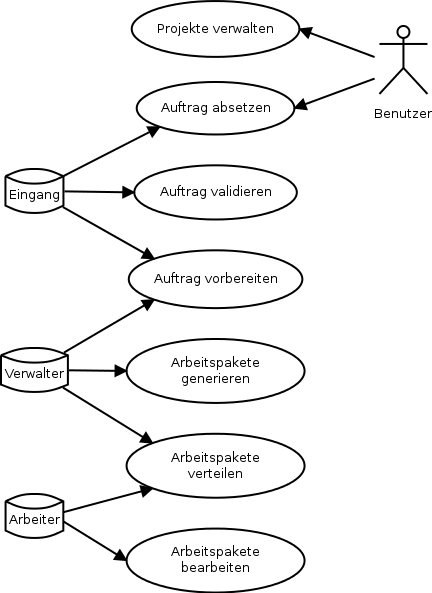
\includegraphics[width=0.7\textwidth]{imageinput/use-case-muss.png}
  \end{center}
  \caption{\"Ubersicht Use Cases Muss}
\end{figure}


\begin{verbatim}
- user wirft build an
- event wirft build an

- build achsen ??

- extensions
  - regressionstest
  - testanalyse

- alte usecases
  - junitxml beispiel
  - stdout beispiel

- neue use-cases
  - workdir diff/tarball
  - auswertung zeitserien <addon>
  - datenanalyse beispiel sommer <addon>
\end{verbatim}

\section{Pflichtenheft ?}

\begin{verbatim}
- programmteile
- siehe andforderungen/funktionen
- tabelle
  - auftragsannahme
  - arbeitspackete
    - generation mit matrix
    - verteilung
    - abarbeitung
  - arbeitsschritte
    - scm
    - prozess
    - ihre datensammlung
      - kontinuierlich
      - dannach?

  - analyse
    - resultate
    - ext regressionsanalyse?
    - ext analysegraph
\end{verbatim}

\section{Unit tests ?}


\begin{verbatim}
- verweis auf grobentwurf?
- hilfskomponenten
- eregeben sich bei impl
\end{verbatim}

\section{funktionale Tests}

\begin{verbatim}
- einzelnen komponenten
  - auftragseingang
  - aftragsvorbereitung
  - auftragsabarbeitung
  - schritte durchlaufen

- schrittypen durchfuehren
 - prozess
 - python ?
 - scm


\end{verbatim}

\section{systemtests}

\begin{verbatim}
- komponentendurchlauf
- durchlauf komplettsystem
- resultate beispiel datenanalyse

\end{verbatim}

